\documentclass[../../main.tex]{subfiles}
\begin{document}
    \subsection{Funciones trigonométricas}
        Considere el siguiente triángulo rectángulo
            \begin{figure}[H]
                \begin{center}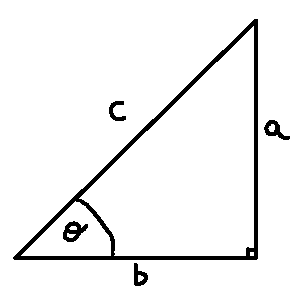
\includegraphics[scale=0.8]{triangulo.pdf}\end{center}
                \caption{Triangulo rectángulo}
            \end{figure}
        donde
            \begin{itemize}
            	\item $\theta$ es un ángulo
            	\item $a$ es el cateto opuesto de $\theta$
            	\item $b$ es el cateto adyacente de $\theta$
            	\item $c$ es la hipótenusa del triangulo.
            \end{itemize}
        Entonces,
            \begin{enumerate}
            	\item $\ds \f \sin \theta = \frac a c$
            	\item $\ds \f \cos \theta = \frac b c$
            	\item $\ds \f \tan \theta = \frac {\f \sin \theta} {\f \cos \theta} = \frac a b$
            	\item $\ds \f \sec \theta = \frac {1} {\f \cos \theta} = \frac c b$
            	\item $\ds \f \csc \theta = \frac {1} {\f \sin \theta} = \frac c a$
            	\item $\ds \f \cot \theta = \frac {1} {\f \tan \theta} = \frac {\f \cos \theta} {\f \sin \theta} = \frac b a$
            \end{enumerate}
    
    \subsection{Desfase}
        \begin{enumerate}
        	\item $\ds \f \sin {x} = \f \cos {x - \frac \pi 2}$
        	\item $\ds \f \cos {-a} = \f \sin {x + \frac \pi 2}$
        \end{enumerate}
        
    \subsection{Paridad}
        \begin{enumerate}
        	\item $\ds \f \sin {-a} = -\f \sin a$
        	\item $\ds \f \cos {-a} = \f \cos a$
        	\item $\ds \f \tan {-a} = - \f \tan a$
        \end{enumerate}


	\subsection{Identidades pitágoras}
        \begin{enumerate}
        	\item $\displaystyle \f {\sin^2} x = 1 - \f {\cos^2} x$
        	\item $\displaystyle \f {\sec^2} x = \f {\tan^2} x + 1$
        	\item $\displaystyle \f {\csc^2} x = \f {\cot^2} x + 1$
        \end{enumerate}
        
    \subsection{Identidades de suma de ángulos}
        \begin{enumerate}
        	\item $\displaystyle \f {\sin} {a+b} = \f {\sin} a \f {\cos} b + \f {\cos} a \f {\sin} b$
        	\item $\displaystyle \f {\cos} {a+b} = \f {\cos} a \f {\cos} b - \f {\sin} a \f {\sin} b$
        	\item $\displaystyle \f {\tan} {a+b} = \frac{\f \tan a + \f \tan b}{1 - \f \tan a \f \tan b}$
        \end{enumerate}
        
    \subsection{Identidades del ángulo doble}
        \begin{enumerate}
        	\item $\displaystyle \f {\sin} {2a} = 2 \f {\sin} a \f {\cos} a$
        	\item $\displaystyle \f {\cos} {2a} = \f {\cos^2} a - \f {\sin^2} a$
        	\item $\displaystyle \f {\tan} {2a} = \frac{2 \f \tan a}{1 - \f {\tan^2} a}$
        \end{enumerate}
    
    \subsection{Identidades del ángulo medio}
        \begin{enumerate}
        	\item $\displaystyle \f {\sin} {\frac a 2} = \pm \sqrt{\frac{1 - \f \cos a} 2}$
        	\item $\displaystyle \f {\cos} {\frac a 2} = \pm \sqrt{\frac{1 + \f \cos a} 2}$
        	\item $\displaystyle \f {\tan} {\frac a 2} = \frac{1 - \f \cos a}{\f \sin a}$
        \end{enumerate}
        
    \subsection{Identidades deducidas desde el ángulo medio}
        \begin{enumerate}
        	\item $\ds \f {\sin^2} x = \frac{1 - \f \cos {2x}} 2$
        	\item $\ds \f {\cos^2} x = \frac{1 + \f \cos {2x}} 2$
        \end{enumerate}
        
    \subsection{Identidades de suma y resta de funciones}
        Defina $\ds s = \frac{a+b}2$ y $\ds r = \frac{a-b}2$. Luego, 
        \begin{enumerate}
        	\item $\ds \f \sin a + \f \sin b = 2 \f \sin s \f \cos r$
        	\item $\ds \f \sin a - \f \sin b = 2 \f \sin r \f \cos s$
        	\item $\ds \f \cos a + \f \cos b = 2 \f \cos s \f \cos r$
        	\item $\ds \f \cos a - \f \cos b = -2 \f \sin s \f \sin r$
        \end{enumerate}
        
    \subsection{Identidades de producto de funciones}
        \begin{enumerate}
        	\item $\ds 2 \f \sin a \f \cos b = \f \sin {a+b} + \f \sin {a-b}$
        	\item $\ds 2 \f \sin a \f \sin b = \f \cos {a-b} - \f \cos {a+b}$
        	\item $\ds 2 \f \cos a \f \sin b = \f \sin {a+b} - \f \sin {a-b}$
        	\item $\ds 2 \f \cos a \f \cos b = \f \cos {a+b} + \f \cos {a-b}$
        \end{enumerate}
    
    \subsection{Función sinusoidal}
        Defina $\ds C = \sqrt{A^2+B^2}$ y $\ds \phi = \f \arctan {\frac B A}$. Luego,
        \begin{align*}
        	A \f \sin {\omega x} + B \f \cos {\omega x} = C \f \sin {\omega x + \phi}
        \end{align*}
    
    \subsection{Teorema del seno}
        \begin{align*}
        	\frac {\f \sin \alpha} a = \frac {\f \sin \beta} b = \frac {\f \sin \gamma} c
        \end{align*}
    
    \subsection{Teorema del coseno}
        \begin{align*}
        	a^2 = b^2 + c^2 - 2bc \f \cos \alpha
        \end{align*}
    
    \subsection{Formas complejas}
        \begin{enumerate}
        	\item $\ds e^{i \theta} = \f \cos{\theta} + i \f \sin{\theta}$
        	\item $\ds \f \sin{\theta} = \frac{e^{i\theta} - e^{-i \theta}}{2i}$
        	\item $\ds \f \cos{\theta} = \frac{e^{i\theta} + e^{-i \theta}}{2}$
        \end{enumerate}

    \subsection{Formas hiperbólicas}
        \begin{enumerate}
        	\item $\ds \f \sinh{x} = \frac{e^{x} - e^{-x}}{2}$
        	\item $\ds \f \cosh{x} = \frac{e^{x} + e^{-x}}{2}$
        	\item $\ds \f \tanh{x} = \frac{e^{x} - e^{-x}}{e^{x} + e^{-x}}$
        \end{enumerate}
    
\end{document}

